\documentclass{beamer}
\usetheme{Warsaw}

\usecolortheme[rgb={0.2,0.4,1}]{structure}
\definecolor{grayColor}{rgb}{0.255,0.25,0.275}
\setbeamercolor{section in head/foot}{bg=grayColor,fg=white}
\setbeamerfont{subsection in head/foot}{size=\small}

\usepackage{tikz}
\usepackage{multimedia}
\usepackage[T1]{fontenc}
\usepackage[utf8]{inputenc}
\setbeamertemplate{footline}[frame number]{}
\setbeamertemplate{navigation symbols}{}


\title{Défier l'ordinateur au Sokoban}
\author{Aymeric BEAUCHAMP\\Dimitri CHAGNEUX\\Valentin LEBLOND\\Baptiste MORI}
\date{Avril 2018}

\begin{document}
\maketitle
\section*{}
\subsection*{Sommaire}
\frame{\tableofcontents}

\section{Notre projet}

\subsection{Objectifs}
\begin{frame}
\begin{itemize}
\item Programmer le jeu Sokoban
\item Ajout d'une interface graphique
\item Résolution automatique de niveau
\item Jouer contre l'ordinateur en temps réel
\end{itemize}
\end{frame}

\subsection{Présentation du sokoban}
\begin{frame} % premier transparent
\begin{columns}
\hspace{0.5cm}
\begin{column}{5cm}
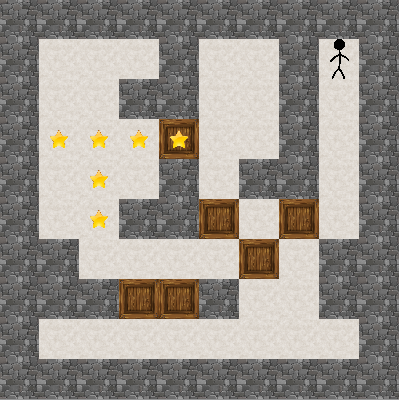
\includegraphics[scale=0.3]{images/sokoban.png}
\end{column}
\begin{column}{6cm}
\begin{itemize}
\item Jeu de réflexion (puzzle)
\item Poussée de caisses
\item Objectif : ranger toutes les caisses
\end{itemize}
\end{column}
\end{columns}
\end{frame}

\subsection{Organisation du projet}
\begin{frame}
\begin{itemize}
\item 1$^{ère}$ séance : conception structure projet + début
\item Puis, 3 groupes :
\begin{enumerate}
\item Version console, gestion de sauvegarde/chargement de fichiers
\item Solveur
\item Interface graphique
\end{enumerate}
\item Décalage entre version console et version graphique
\item Rassemblement pour la finalisation
\end{itemize}
\end{frame}

\section{Architecture du projet}
\subsection{Packages utilisés}
\begin{frame}
\begin{center}
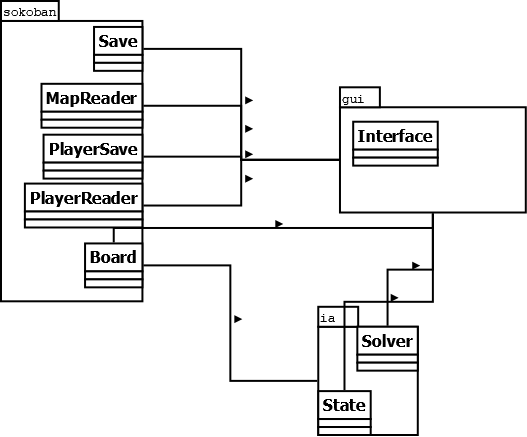
\includegraphics[scale=0.3]{images/packages.png}
\end{center}
\end{frame}

\section{Eléments techniques}
\subsection{Deadlocks}

\begin{frame}

\begin{block}{Définition}
Une caisse en deadlock, est une caisse qu'on ne peut plus déplacer directement ou indirectement. Le jeu est donc bloqué.
\end{block}
\vspace{0.5cm}
\begin{center}
\begin{columns}
\begin{column}{4cm}
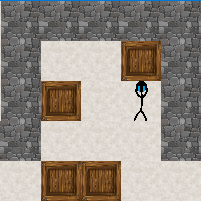
\includegraphics[scale=0.7]{images/deadlock1.PNG}
\end{column}
\begin{column}{4cm}
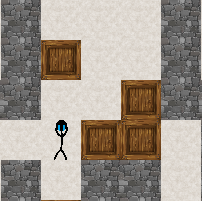
\includegraphics[scale=0.7]{images/deadlock2.PNG}
\end{column}
\end{columns}
\end{center}
\end{frame}

\begin{frame}
\begin{center}
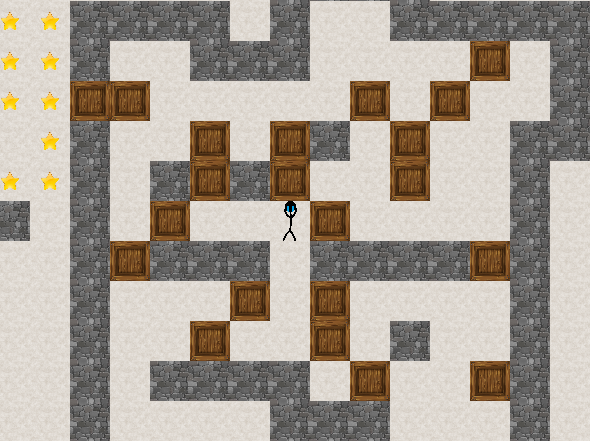
\includegraphics[scale=0.65]{images/deadlock3.PNG}
\end{center}
\end{frame}

\subsection{Résolution automatique}
\begin{frame}
\begin{columns}
\begin{column}{5cm}
Déplacement automatisé
\begin{itemize}
\item Algorithme A*
\end{itemize}
\movie[loop,autostart]{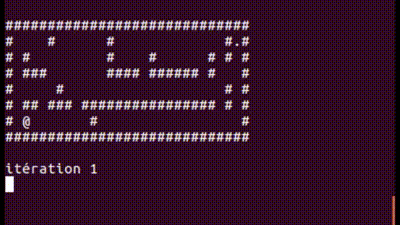
\includegraphics[scale=0.4]{images/gif/frame_0.png}}{images/dep.flv}
\end{column}
\pause
\begin{column}{5cm}
Solveurs
\begin{itemize}
\item $1^{er}$ solveur inspiré de minmax (peu efficace)
\item $2^{nd}$ solveur basé sur A*
\end{itemize}
Heuristiques :
\begin{itemize}
\item distances de Manhattan
\item distance de Hamming
\end{itemize}
\end{column}
\end{columns}
\end{frame}

\begin{frame}
\begin{figure}[!h]
\centering
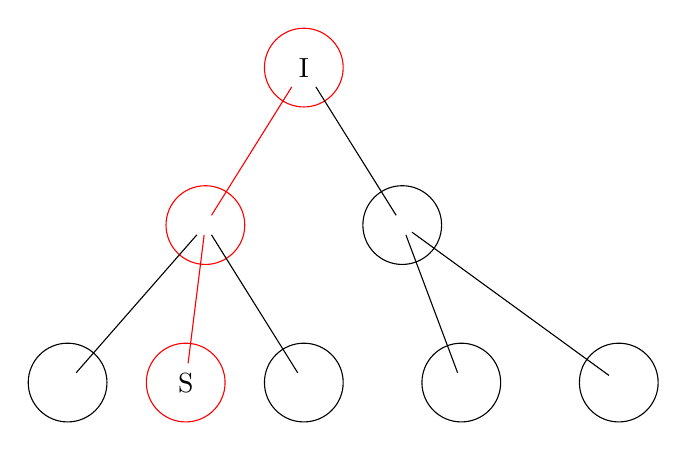
\begin{tikzpicture}
\node (dep) at (0,0) {I};
\draw[color=red] (0,0) circle(0.5);
\node (e1) at (-1.25,-2) {};
\draw[color=red] (-1.25,-2) circle(0.5);
\node (e2) at (1.25,-2) {};
\draw (1.25,-2) circle(0.5);
\node (e3) at (-3,-4) {};
\draw (-3,-4) circle(0.5);
\node (e4) at (-1.5,-4) {S};
\draw[color=red] (-1.5,-4) circle(0.5);
\node (e5) at (0,-4) {};
\draw (0,-4) circle(0.5);
\node (e6) at (2,-4) {};
\draw (2,-4) circle(0.5);
\node (e7) at (4,-4) {};
\draw (4,-4) circle(0.5);
\draw[color=red] (dep) -- (e1);
\draw (dep) -- (e2);
\draw (e1) -- (e3);
\draw[color=red] (e1) -- (e4);
\draw (e1) -- (e5);
\draw (e2) -- (e6);
\draw (e2) -- (e7);
\end{tikzpicture}
\end{figure}
\end{frame}

\begin{frame}
\frametitle{Démonstration}
\movie[autostart]{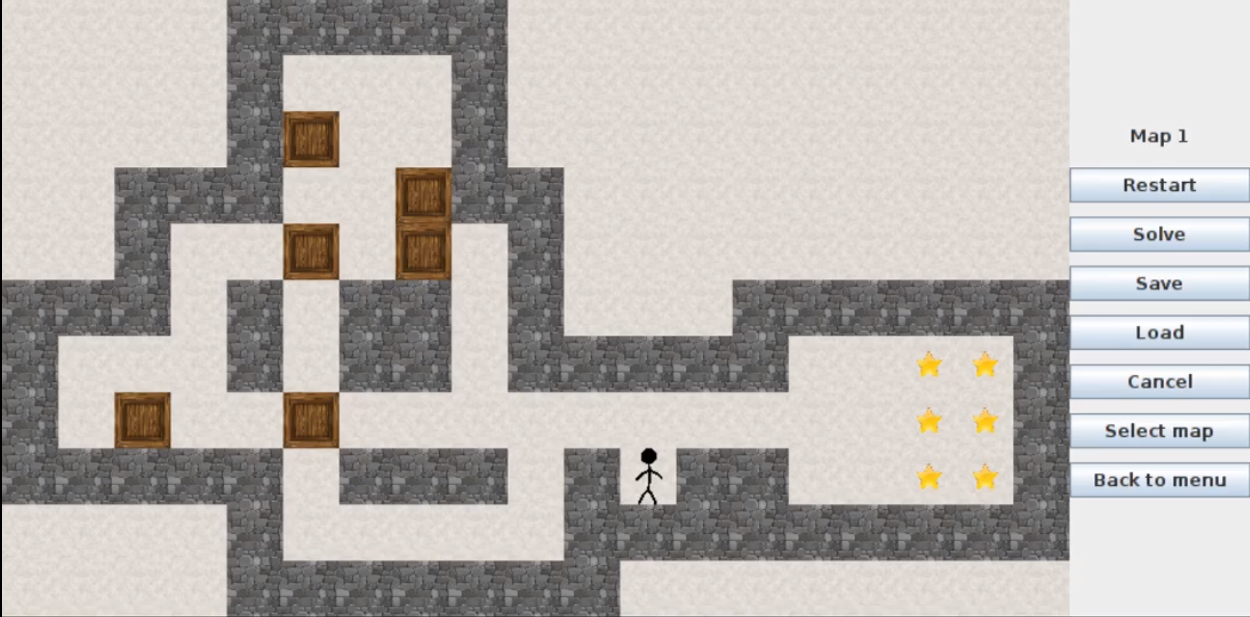
\includegraphics[scale=0.25]{images/im_solver.png}}{images/solveur.flv}
\end{frame}

\subsection{Fonctionnement anytime}
\begin{frame}
Deux threads :
\begin{itemize}
\item Thread principal en charge de l'interface graphique et de l'écoute des entrées joueur
\item Thread auxiliaire pour la recherche de chemin
\end{itemize}
Interruption du thread auxiliaire lors du déplacement du joueur et mise à jour du canvas de l'ordinateur
\end{frame}

\section{Expérimentations et usages}
\subsection{Performance du solveur}
\begin{frame}
  Série de niveaux Sokoban junior par Laura Wheeler (58 niveaux)\\
  \centering
  \begin{tabular}{|l|c|c|}
  \hline
  Heuristique                          & Hamming   & Manhanttan \\
  \hline
  Limite de temps                      & 5 minutes & 10 minutes \\
  \hline
  Limite d'états en mémoire            & 175 000   & 180 000    \\
  \hline
  Niveaux résolus                      &    34     &    12      \\
  \hline
  Niveaux considérés comme insolubles  &    0      &    20      \\
  \hline  
  \end{tabular}
\end{frame}

\section{Conclusion}
\subsection{Réalisation des objectifs}
\begin{frame}
\begin{itemize}
\item Globalement les objectifs ont été réalisés
\item Première expérience de conception logicielle
\item Travail en groupe
\end{itemize}
\end{frame}

\subsection{Améliorations possibles}
\begin{frame}
\begin{itemize}
\item Solveur
\begin{itemize}
\item Réduire la mémoire utilisée
\item Trouver de meilleurs chemins
\end{itemize}
\item Meilleur comportement de l'ordinateur en mode \textit{anytime}
\item Ajouter des éléments de gameplay (téléporteurs, etc.)
\item Statistiques (temps de résolution, nombre de coups)
\end{itemize}
\end{frame}

\end{document}
